\section{Simulations}


\subsection{System Characterisation}

After  a system's  step  response  has  been  measured,  it  is  necessary  to
characterise  and  determine  its  properties before it's possible  to  fit  a
transfer function to it. The method  of  characterisation used here is to find
the point of inflection in the measured step response, through which a tangent
is placed.  The  tangent's  intersection  points  with  the  lower  and  upper
horizontal bounds  are used to determine the dead time $T_u$ and the rise time
$T_g$.  Further, the amplitude $K_s$ of the step response can  be  determined.
This process is illustrated in figure \ref{fig:tu-tg-example}.

\begin{figure}[t]
    \centering
    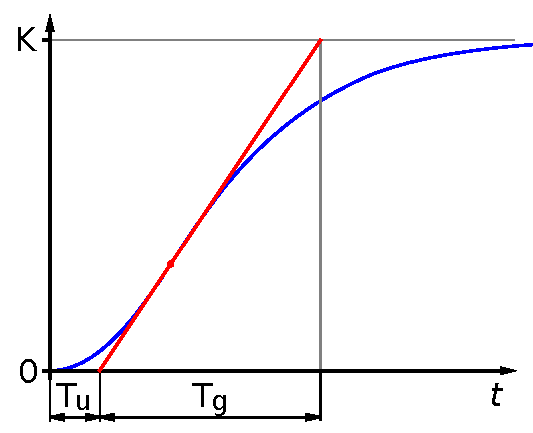
\includegraphics[width=\imagewidth]{images/tu_tg_example}
    \caption{Example step response of a system and measurement of the angle of inflection for determining $K_s$, $T_u$ and $T_g$. Image taken from Wikipedia\cite{ref:tu-tg}.}
    \label{fig:tu-tg-example}
\end{figure}

It is important to note that this method  of  characterisation  is  valid  for
systems  with  an  order of at least  2  that  don't  exhibit  any  overshoot.

\begin{figure}[t]
    \centering
    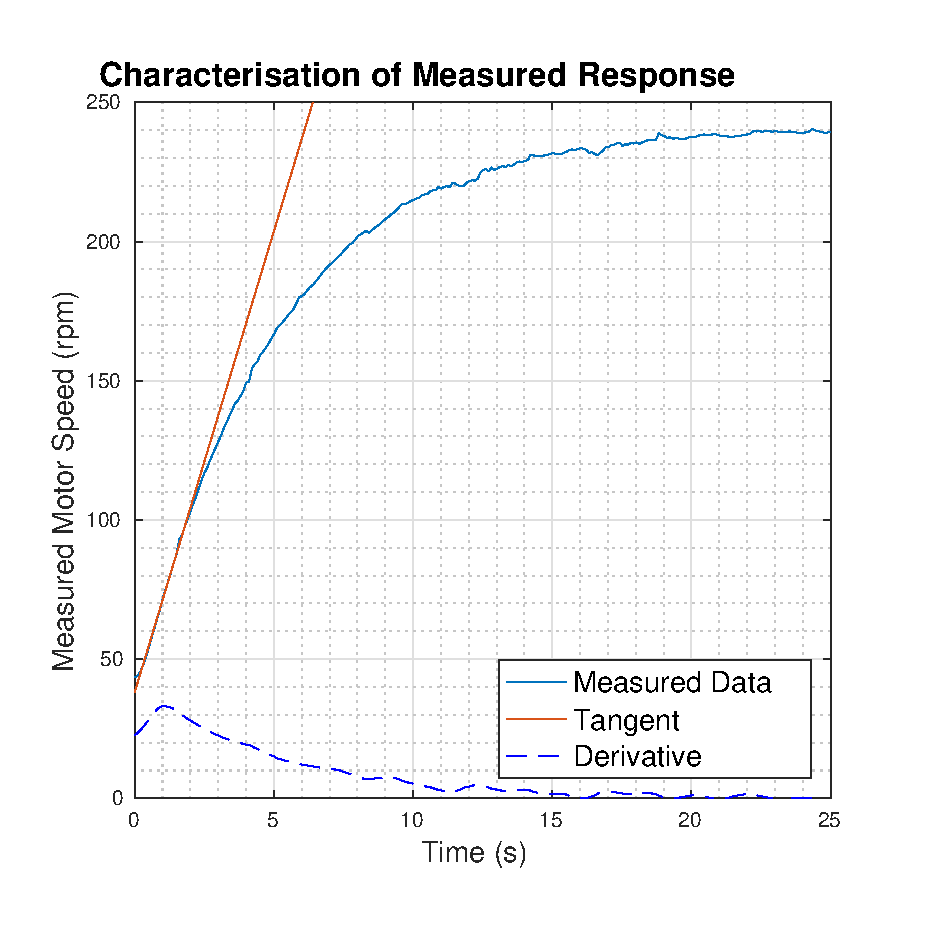
\includegraphics[width=\imagewidth]{images/characterisation}
    \caption{Calculated tangent of measured step response data.}
    \label{fig:characterisation}
\end{figure}

Using  MATLAB, the measured step response from the lab experiment is smoothed,
the derivative is computed to find the point of inflection, and the tangent is
calculated.   The    results    of    this    are    visualised    in   figure
\ref{fig:characterisation}.

Regarding the parameter $K_s$, a common pitfall is to  say  that  $K_s$ is the
total  change in the step response. This  statement  is  in  fact  false,  but
happens to yield the correct value as long as the input step  function  has an
amplitude of $1$, which unfortunately is the only case studied in the majority
of theory lectures. The parameter $K_s$ is in fact the total change in  output
divided by the total change in input:

\begin{equation}
    K_s = \frac{\Delta K_{out}}{\Delta K_{in}}
\end{equation}

The calculated values of $T_u$, $T_g$ and $K_s$ turn out to be:

\begin{align*}
    T_u &= 0.1655 \\
    T_g &= 5.9602 \\
    K_s &= 197.42
\end{align*}


\subsection{System Identification using Dead-Time and PT1 elements}
\label{sec:ident_Tt_PT1}

It  is  known  that the motor has a dead-time built in, and by looking at  the
step  response, one can say that it looks like a PT1 element might be  a  good
approximation.

The dead time element and its Laplace transform is:

\begin{equation}
    F_{T_t}(s) = \laplace{\{\epsilon(t)(t-T_t)} = e^{-sT_t}\}
\end{equation}

The PT1 lag element and its Laplace transform is:

\begin{equation}
    F_{PT1}(s) = \laplace{\{\epsilon(t)e^{-sT_g}}\}
\end{equation}

These two elements are combined to obtain the model we will use to approximate
the measured step response:

\begin{equation}
    G_1(s) = F_1(s) \cdot F_2(s) = e^{-sT_t} \frac{K_s}{sT_g+1}
\end{equation}

By  plugging  in  the  parameters  obtained  from the characterisation step in
section  \ref{sec:sim:characterisation}  (dead-time  $T_t=T_u$)  we obtain the
following transfer function:

\begin{equation}
    G_1(s) = e^{-0.165*s}\frac{24.68}{5.96s + 1}
\end{equation}

Figure  \ref{fig:Tt_PT1_step}  shows  the  step  response  of  the  calculated
transfer function $G_1(s)$ and compares it to the measured step response. It's
pretty  close, perhaps the parameter $T_g$ can be adjusted so it rises faster.
When doing this, however, the function no longer matches  the measured data at
the  beginning  where  it  starts  rising.  It's  possible therefore that  the
measured system  is of higher order. Adding more PT1 elements to our model can
help make the approximation more  exact, but for this experiment we will stick
to a single PT1 element.

By  looking  at  the  Bode-Diagram  of  the   model   $G_1(s)$   (see   figure
\ref{fig:Tt_PT1_bode})  it  is  very  easy  to  determine  the  critical  gain
$K_{s,crit}$. This is the  point at which the phase exceeds \SI{180}{\degree}.
The amplitude at  this  point  is  about  \SI{-36}{\decibel}, which means that
$K_{s,crit}=\SI{36}{\decibel}$, or:

\begin{equation}
    K_{s,crit} = 10^{\frac{\SI{36}{\decibel}}{20}} \approx 63.1
\end{equation}

\begin{figure}[h]
    \centering
    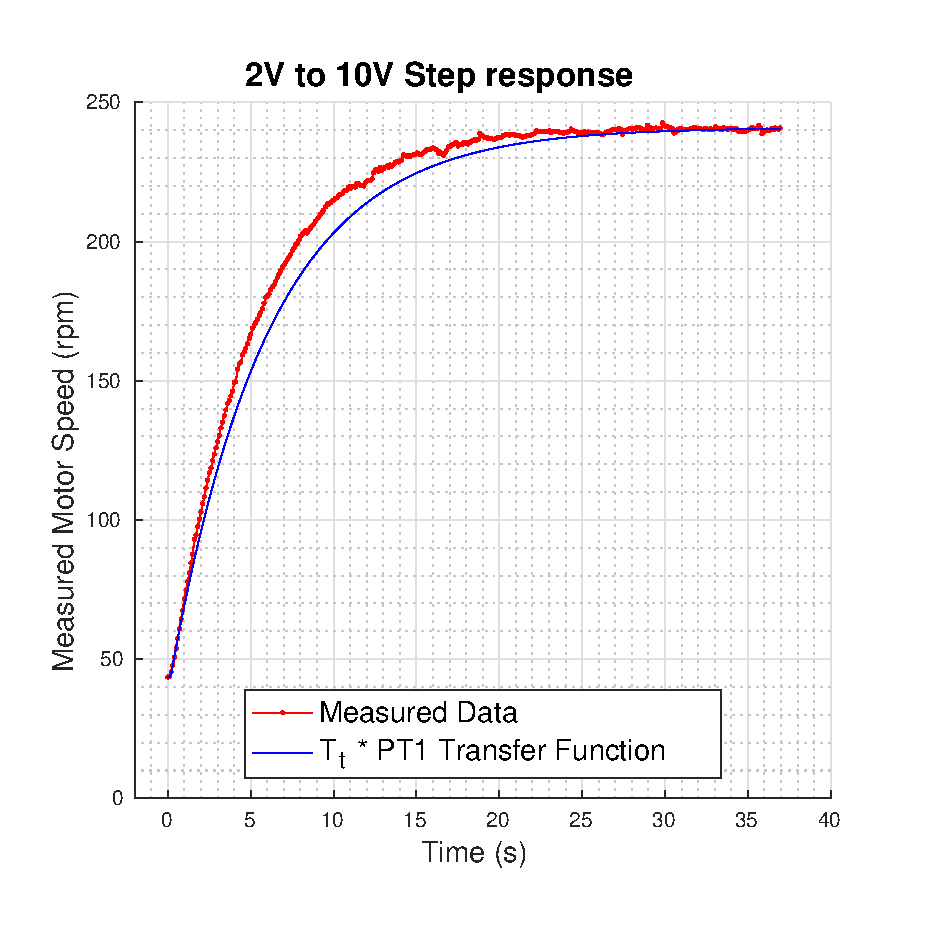
\includegraphics[width=\imagewidth]{images/Tt_PT1}
    \caption{Step response comparison of calculated system $G_1(s)$ and the measured step response.}
    \label{fig:Tt_PT1_step}
\end{figure}

The  closed  loop  transfer  function  of  $G_1(s)$  with  a  P-controller  is
constructed:

\begin{equation}
    T(s) = \frac{H(s)G_1(s)}{1 + H(s)G_1(s)}
\end{equation}

Where  $H(s)$  is  simply  the  P controller. By setting $H(s)=K_{p,crit}$ and
simulating a step  response,  we  obtain  a  system  that exhibits an undamped
oscillation (see  figure \ref{fig:Tt_PT1_tcrit}). Determining $\tau_{crit}$ is
now simply a matter of measuring two points in this graph.

\begin{equation}
    \tau_{crit} \approx 0.66
\end{equation}

\begin{figure}[h]
    \centering
    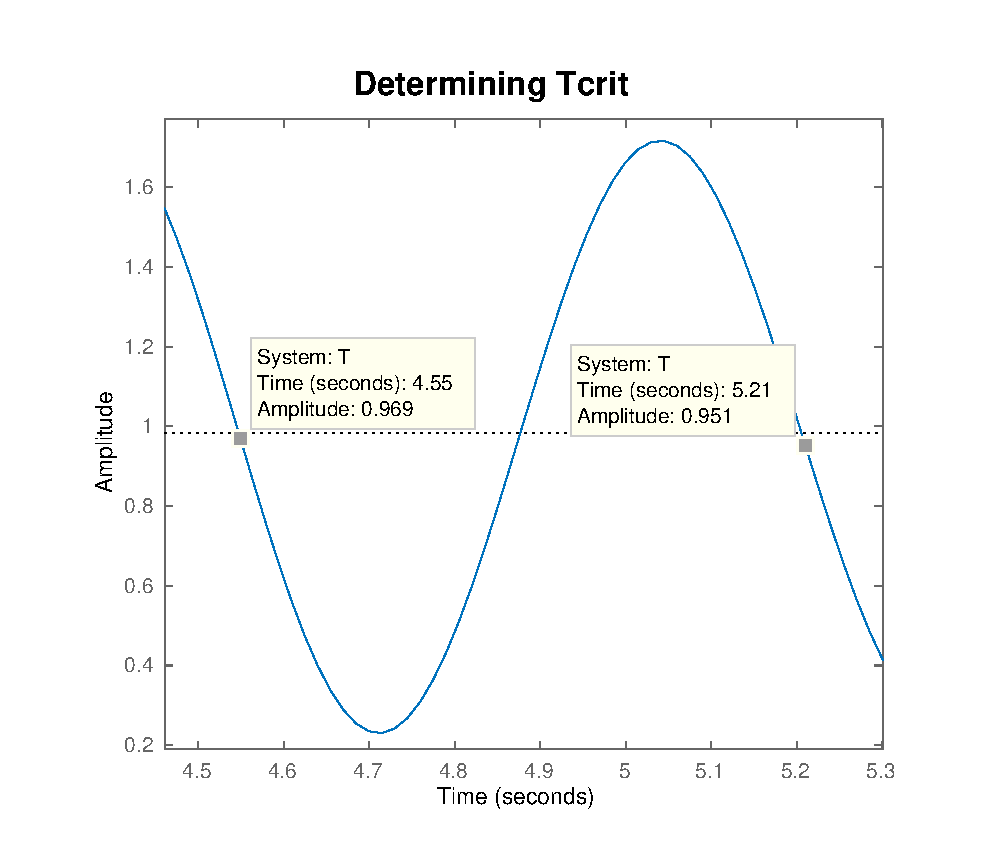
\includegraphics[width=\imagewidth]{images/tcrit}
    \caption{Step response of the closed loop transfer function with $K_p=K_{p,crit}$}
    \label{fig:Tt_PT1_tcrit}
\end{figure}

\begin{figure}[h]
    \centering
    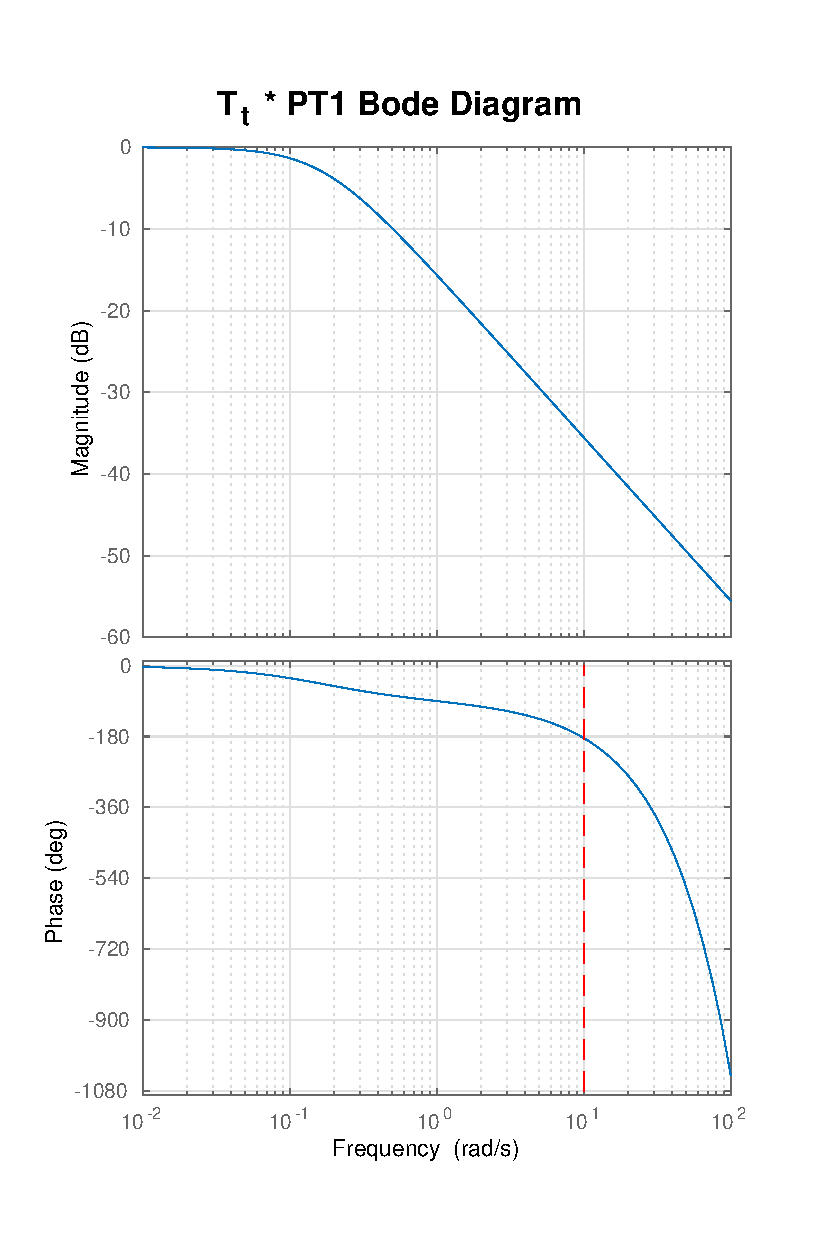
\includegraphics[width=\imagewidth]{images/Tt_PT1_bode}
    \caption{Bode-Plots of the model $G_1(s)$. The phase exceeds \SI{180}{\degree} at about \SI{-36}{\decibel}}
    \label{fig:Tt_PT1_bode}
\end{figure}



\begin{figure}
    \centering
    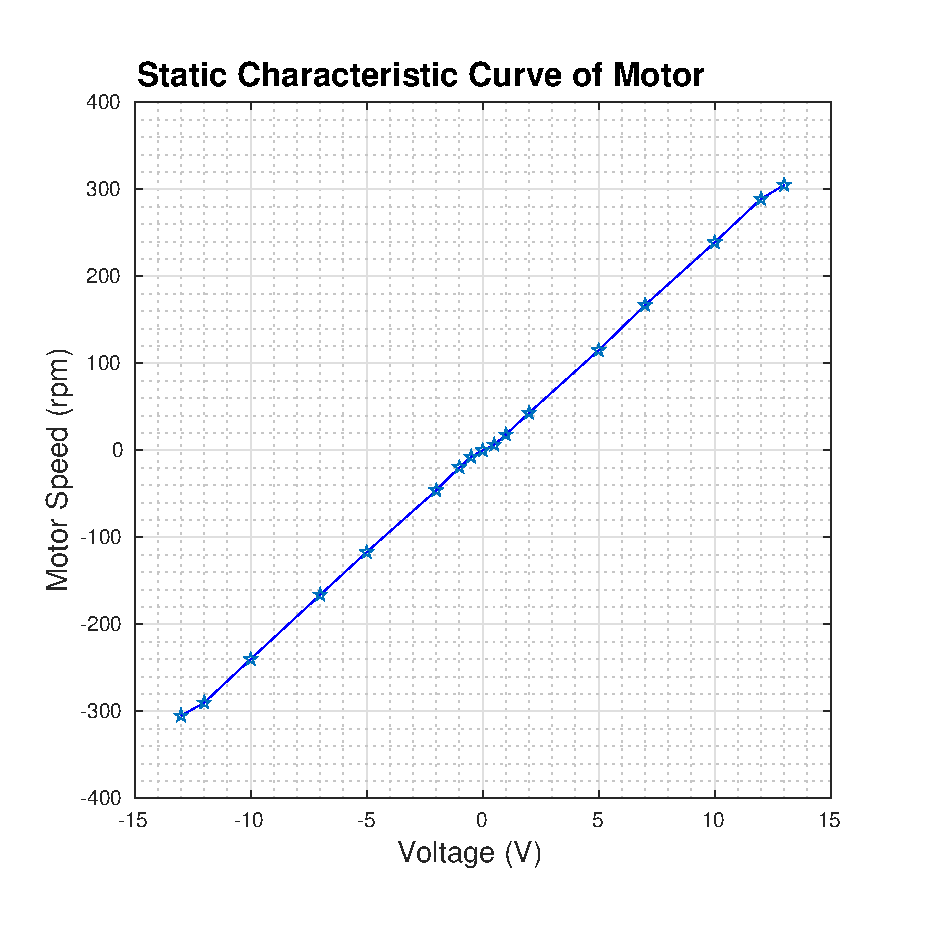
\includegraphics[width=\linewidth]{images/static_cc}
    \caption{XXX}
\end{figure}

\begin{figure*}
    \centering
    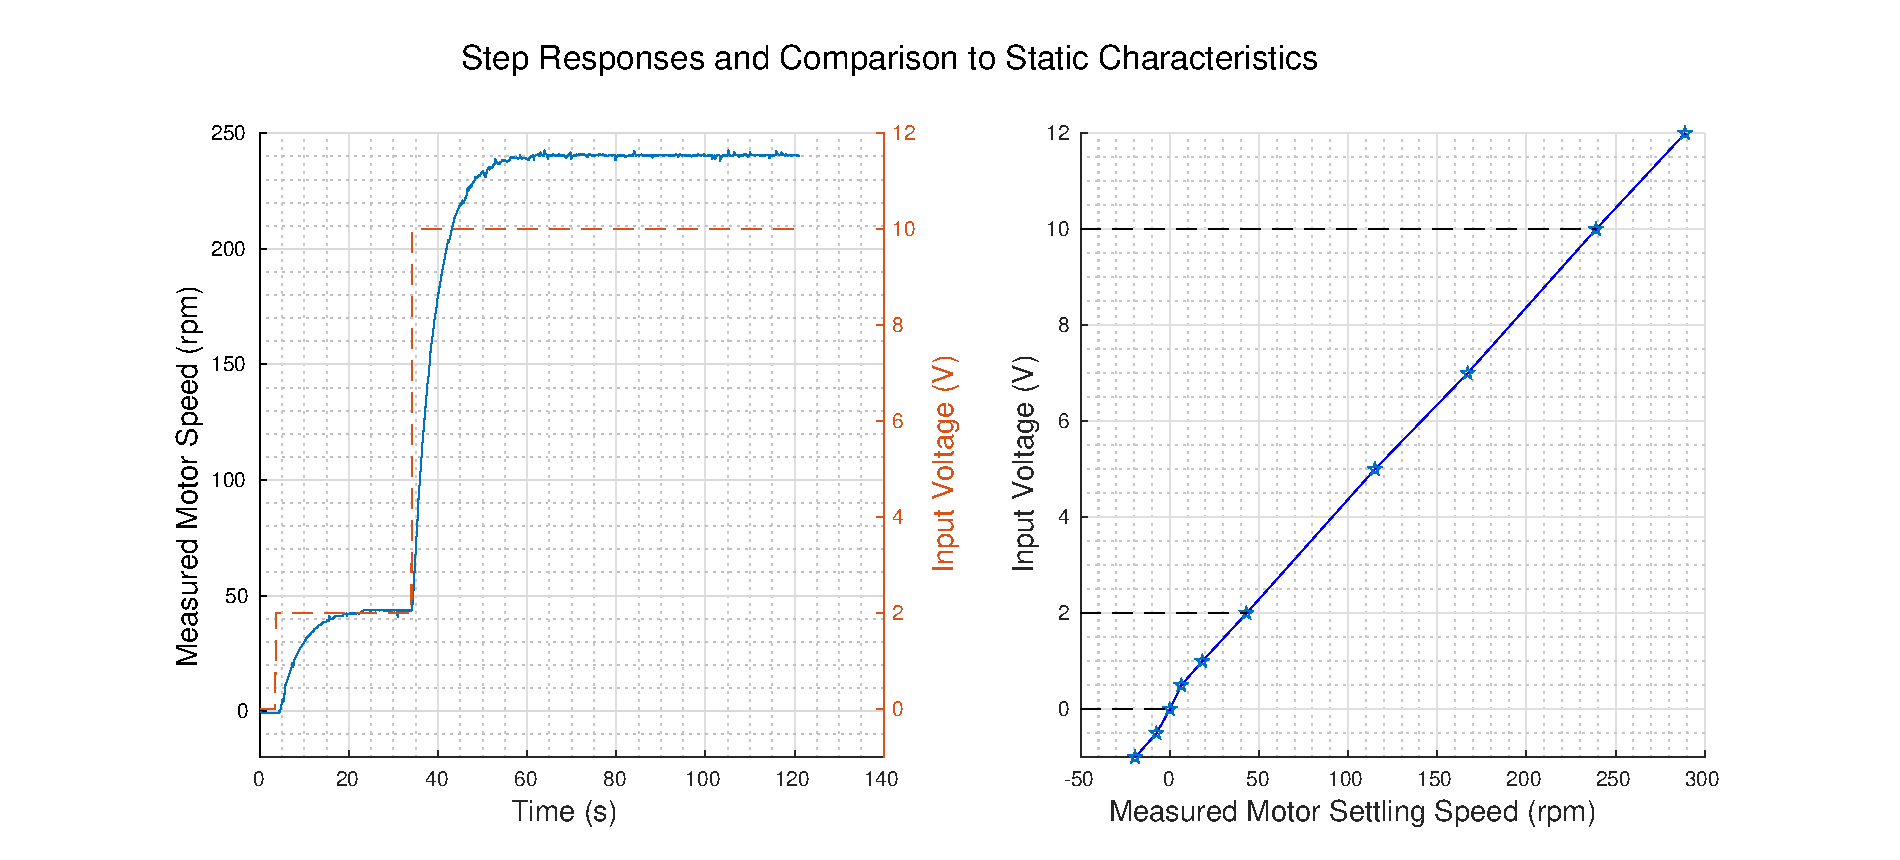
\includegraphics[width=\linewidth]{images/step_response}
    \caption{XXX}
\end{figure*}

\begin{figure}
    \centering
    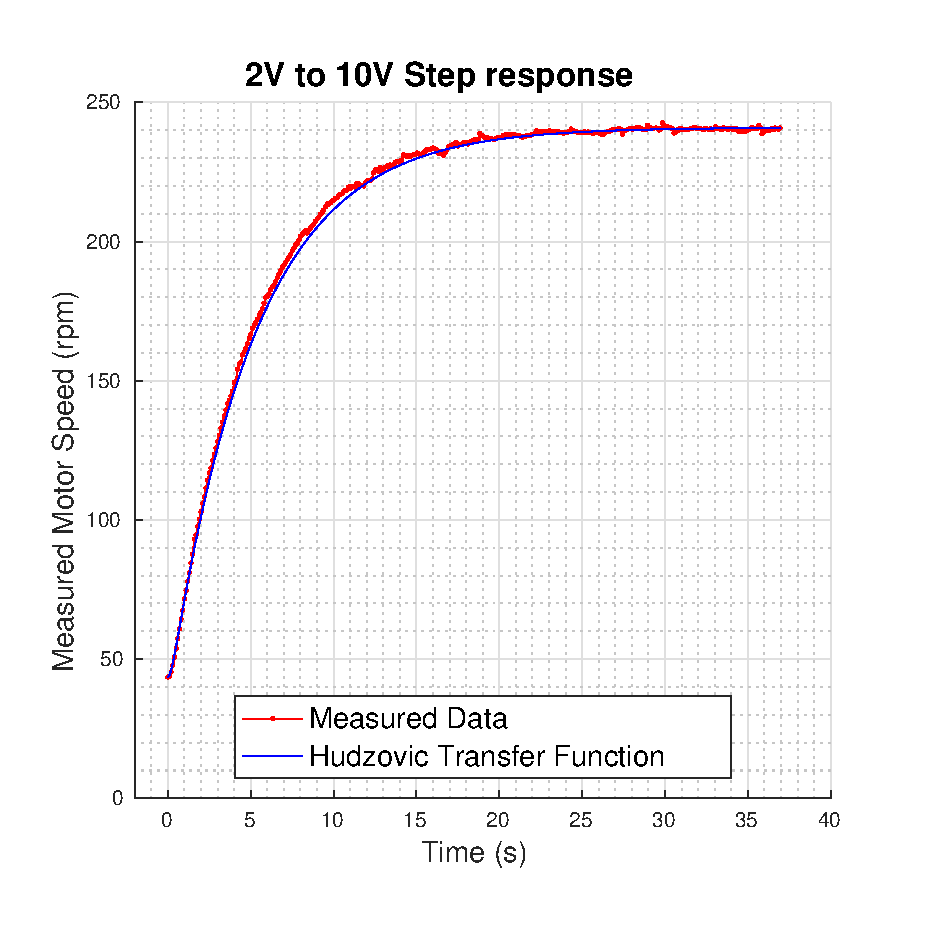
\includegraphics[width=\linewidth]{images/hudzovic}
    \caption{XXX}
\end{figure}


\begin{figure}
    \centering
    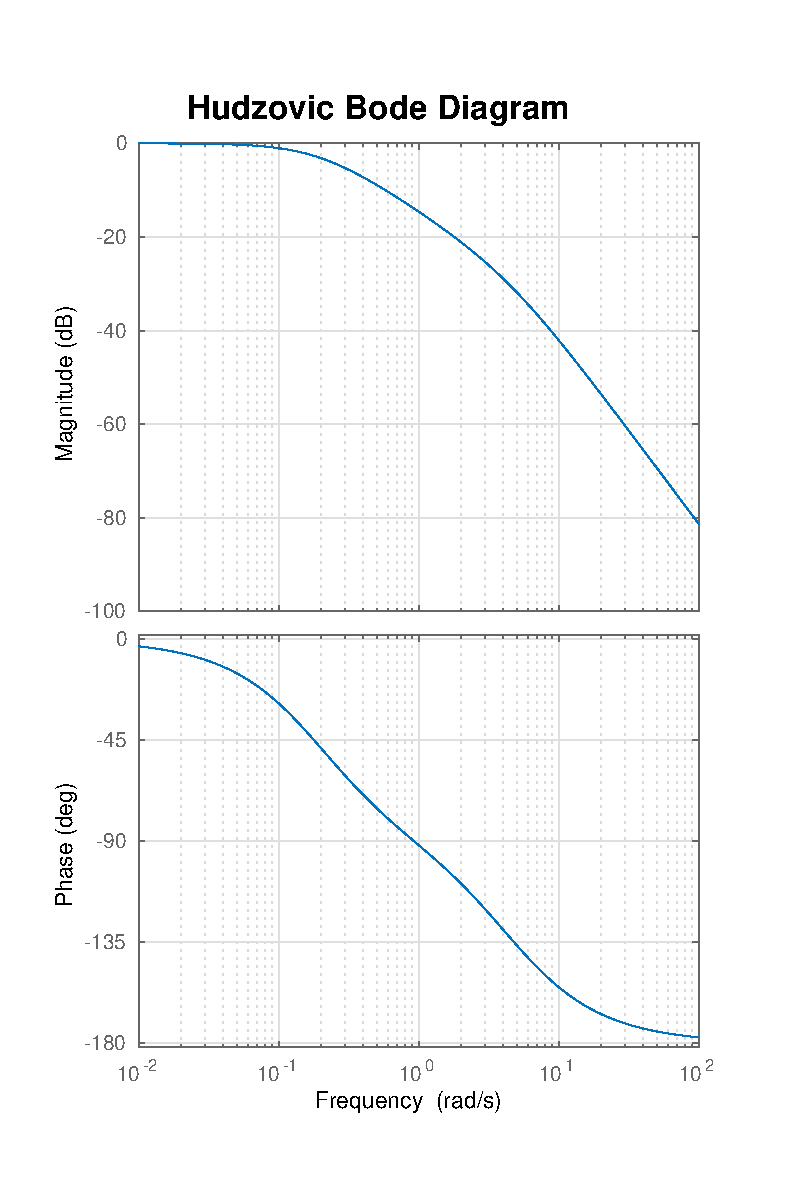
\includegraphics[width=\linewidth]{images/hudzovic_bode}
    \caption{XXX}
\end{figure}

\begin{figure}
    \centering
    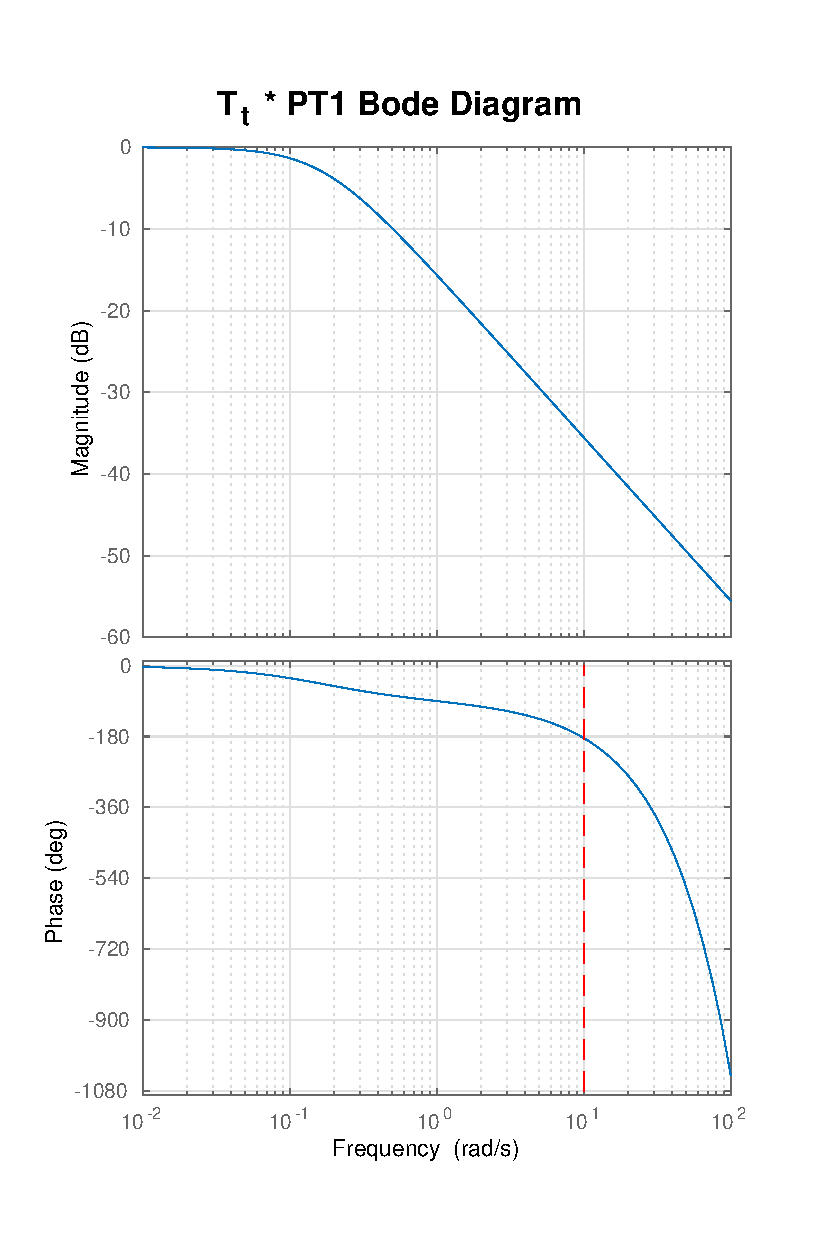
\includegraphics[width=\linewidth]{images/Tt_PT1_bode}
    \caption{XXX}
\end{figure}

\subsection{Simulation with simulink}
A simulation were done in simulink to compare the tracking behavior between simulation and experiment.
First we determine the parameter of the controller with the simulation in the picture 1.
The best value for the $PT_{1}$ we determine were $5.947$
so our $PT_{1}$ element is from the form:
\begin{equation}
G(s) = \frac{1}{5.947s+1}
\end{equation}



